\subsection{Index sensitivity}\label{index-sensitivity}

\Needspace*{12\baselineskip}\small\setlength{\tabcolsep}{3pt}\begin{longtable}[]{@{}
  >{\raggedright\arraybackslash}p{(\linewidth - 12\tabcolsep) * \real{0.1429}}
  >{\raggedright\arraybackslash}p{(\linewidth - 12\tabcolsep) * \real{0.1429}}
  >{\raggedright\arraybackslash}p{(\linewidth - 12\tabcolsep) * \real{0.1429}}
  >{\raggedright\arraybackslash}p{(\linewidth - 12\tabcolsep) * \real{0.1429}}
  >{\raggedright\arraybackslash}p{(\linewidth - 12\tabcolsep) * \real{0.1429}}
  >{\raggedright\arraybackslash}p{(\linewidth - 12\tabcolsep) * \real{0.1429}}
  >{\raggedright\arraybackslash}p{(\linewidth - 12\tabcolsep) * \real{0.1429}}@{}}
\caption{Baseline level and attribution shares under six inequality indices. Every row was recomputed for its own index against its own baseline; no coalition value or share is transferred between indices. Shares within a row sum to one hundred by exhaustiveness. A negative preference share means that equalizing preferences alone would raise that index, which is a property of this exhaustive two-group game with a nonnegative index and is explained in the text.}\tabularnewline
\toprule\noalign{}
\begin{minipage}[b]{\linewidth}\raggedright
Population and index
\end{minipage} & \begin{minipage}[b]{\linewidth}\raggedright
Baseline level
\end{minipage} & \begin{minipage}[b]{\linewidth}\raggedright
Preferences (per cent)
\end{minipage} & \begin{minipage}[b]{\linewidth}\raggedright
Access
\end{minipage} & \begin{minipage}[b]{\linewidth}\raggedright
Earning opportunities
\end{minipage} & \begin{minipage}[b]{\linewidth}\raggedright
Resources and needs
\end{minipage} & \begin{minipage}[b]{\linewidth}\raggedright
Access + earnings
\end{minipage} \\
\midrule\noalign{}
\endfirsthead
\toprule\noalign{}
\begin{minipage}[b]{\linewidth}\raggedright
Population and index
\end{minipage} & \begin{minipage}[b]{\linewidth}\raggedright
Baseline level
\end{minipage} & \begin{minipage}[b]{\linewidth}\raggedright
Preferences (per cent)
\end{minipage} & \begin{minipage}[b]{\linewidth}\raggedright
Access
\end{minipage} & \begin{minipage}[b]{\linewidth}\raggedright
Earning opportunities
\end{minipage} & \begin{minipage}[b]{\linewidth}\raggedright
Resources and needs
\end{minipage} & \begin{minipage}[b]{\linewidth}\raggedright
Access + earnings
\end{minipage} \\
\midrule\noalign{}
\endhead
\bottomrule\noalign{}
\endlastfoot
Single-adult, Gini & 0.193596 & 9.88 & 49.16 & 6.76 & 34.20 & 55.92 \\
Single-adult, Atkinson(1) & 0.060788 & -7.21 & 55.12 & 5.18 & 46.90 & 60.31 \\
Single-adult, Atkinson(2) & 0.115514 & -6.83 & 58.49 & 4.77 & 43.57 & 63.27 \\
Single-adult, GE(0) & 0.062714 & -7.86 & 55.42 & 5.26 & 47.19 & 60.67 \\
Single-adult, GE(1) & 0.065890 & -7.59 & 49.64 & 5.22 & 52.73 & 54.87 \\
Single-adult, GE(2) \(=CV^2/2\) & 0.153963 & -8.52 & 40.89 & 4.78 & 62.86 & 45.67 \\
Couple, Gini & 0.132465 & 4.85 & 8.23 & 35.72 & 51.20 & 43.95 \\
Couple, Atkinson(1) & 0.030197 & 2.52 & 6.38 & 30.50 & 60.60 & 36.88 \\
Couple, Atkinson(2) & 0.055239 & 2.74 & 6.94 & 33.10 & 57.21 & 40.05 \\
Couple, GE(0) & 0.030663 & 2.55 & 6.40 & 30.48 & 60.57 & 36.88 \\
Couple, GE(1) & 0.034637 & 2.27 & 5.70 & 27.09 & 64.94 & 32.79 \\
Couple, GE(2) \(=CV^2/2\) & 0.088142 & 2.03 & 4.95 & 22.87 & 70.16 & 27.82 \\
\end{longtable}

\begin{figure}[H]
\centering
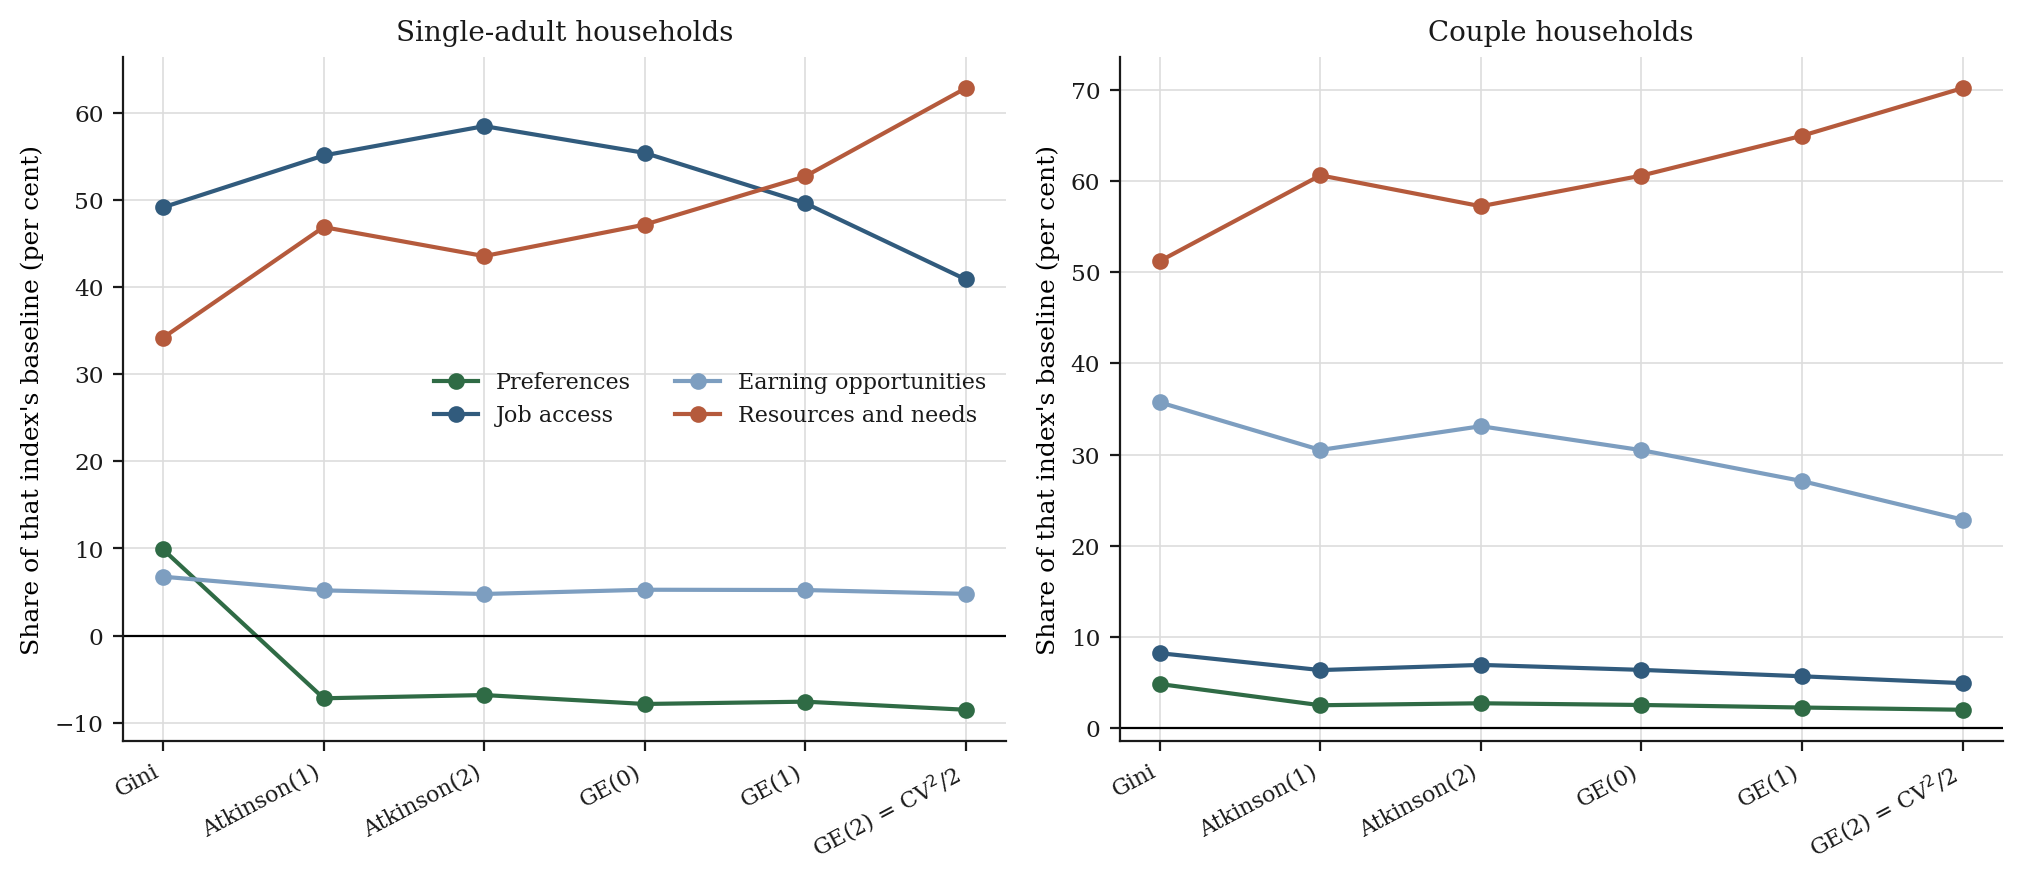
\includegraphics[width=0.95\linewidth,height=\textheight,keepaspectratio,alt={Attribution shares under six inequality indices. Each index keeps its own coalition values and its own allocation. Access exceeds earning opportunities for single adults under all six and the ordering reverses for couples under all six; the singles preference share changes sign outside the Gini.}]{figures/v5/figV05_six_index_shares.png}
\caption{Attribution shares under six inequality indices. Each index keeps its own coalition values and its own allocation. Access exceeds earning opportunities for single adults under all six and the ordering reverses for couples under all six; the singles preference share changes sign outside the Gini.}
\end{figure}

Each index keeps its own coalition values and its own allocation; nothing is transferred between rows. Read carefully, the table supports the following and not more.

\begin{itemize}
\tightlist
\item
  Job access exceeds earning opportunities for single adults under all 6 indices, and earning opportunities exceed access for couples under all 6. This is the robust ordering and it is the one we emphasise.
\item
  Job access alone exceeds resources and needs for single adults under 4 of the six; GE(1) and GE(2) are the exceptions.
\item
  Access and earning opportunities together exceed resources and needs for single adults under 5 of the six, with GE(2) the exception.
\item
  Resources and needs are the largest of the four components for couples under all 6 indices.
\item
  The single-adult preference share is positive for the Gini and negative under the other 5 indices. The preference contribution is therefore \emph{not} a metric-invariant conclusion, and the statement that preferences account for about ten per cent of inequality is a statement about the Gini on the raw basis under the female-primary reference, not a general one.
\end{itemize}

These are descriptive rankings of point estimates. Parameter intervals are reported for the Gini shares only, and we do not convert any of these orderings into a claim of statistical significance.

